This exercise has been completed in the attached \textit{Regression.ipynb} Jupyter Notebook, and \textit{linreg.py} python file, which is imported by the Notebook. The most relevant bits of source code can be seen here as well, though all comments are left out. The \textit{linreg.py} file is a modified version of the given file of the same name. Code not included here is simply unmodified. The full source code is in the notebook, along with comments:\\
\begin{verbatim}
def hsig(xbar,xn,sigma):
    return np.exp(-(np.linalg.norm(xbar-xn)**2)/(2*sigma**2))

def nonlinfit(self, X, t, xbar, sigma):
        X = numpy.array(X).reshape((len(X), -1))
        t = numpy.array(t).reshape((len(t), 1))
        ones = numpy.ones((X.shape[0], 1))
        X = numpy.concatenate((ones, X), axis=1)
        diag = self.lam * len(X) * numpy.identity(X.shape[1])
        h = np.zeros((X.shape[0],X.shape[0]))
        for j in range(X.shape[0]):
            h[j,j] = hsig(X[j], xbar, sigma)
        a = X.T @ h @ X + diag
        b = X.T @ h @ t
        self.w = numpy.linalg.solve(a,b)
\end{verbatim}
To find $\hat{w}(\bar{x})$ we first have to derive the function given. First off, we will write it as a function of matrices and vectors:
$$
\underset{w}{argmin} \frac{1}{N} \sum_{n=1}^N h_\sigma(\bar{x},x_n)(w^Tx_n-t_n)^2 = \nabla_w \frac{1}{N}h_\sigma\Big((Xw-t)^T (Xw-t)\Big)
$$
$$
\nabla_w \frac{1}{N}h_\sigma\Big((Xw^T-t^T) (Xw-t)\Big)
$$
$$
\nabla_w \frac{1}{N}h_\sigma\Big((Xw)^TXw-t^TXw-(Xw)^T t + t^Tt\Big)
$$
$$
\nabla_w \frac{1}{N}h_\sigma\Big(w^TX^TXw- 2w^TX^Tt + t^Tt\Big)
$$
$$
\nabla_w \Big(\frac{1}{N} w^TX^Th_\sigma Xw - \frac{2}{N} w^TX^Th_\sigma t + \frac{1}{N} t^Th_\sigma t\Big)
$$
$$
\frac{2}{N}X^Th_\sigma Xw - \frac{2}{N}X^Th_\sigma t
$$
$$
X^Th_\sigma Xw - X^Th_\sigma t = 0
$$
$$
X^Th_\sigma Xw = X^Th_\sigma t
$$
This expression is what we solve for in the function, as $a$ and $b$ respectively.\\
It should be noted that the numerical problems described in the assignment already happen when $\sigma = 0.1$ on my pc. We instead run it with $\sigma = 0.3$ to give a similar effect.\\
We see that the outcome we predicted in $4a$ was true. Higher values of sigma leads to each point having a smaller effect on the overall look of the model, and lower values do the opposite. We see that when we run the function with low values of sigma, we get significant overfitting that is not useful in a model. When we go up to higher values we see that the resulting graph flattens out. Eventually, when we try a $\sigma = 100$ we see that it resembles the linear regression shown earlier in the given notebook. Plots showing graphs for high sigma values are in the attached Notebook.\\
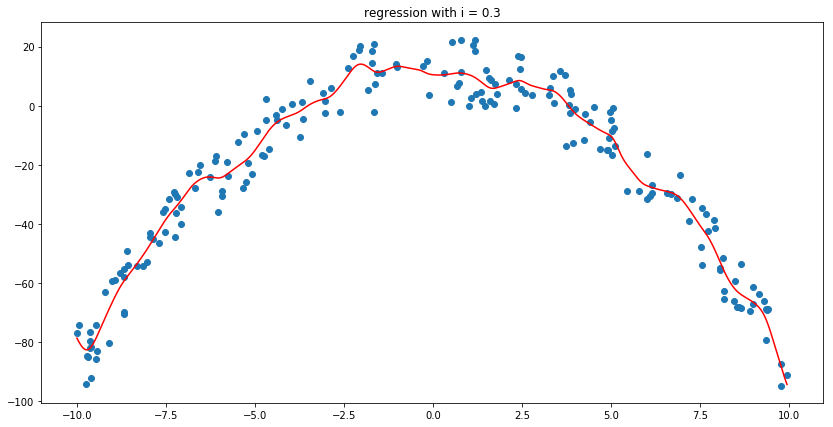
\includegraphics[width=\linewidth]{4b1.png}\\
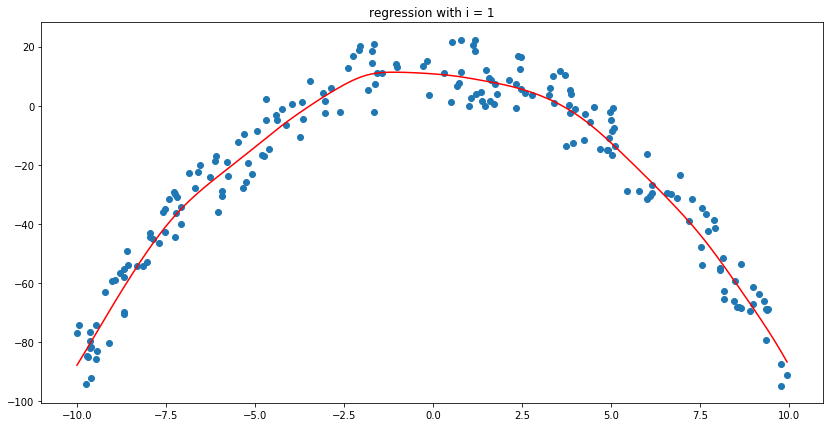
\includegraphics[width=\linewidth]{4b2.png}\\
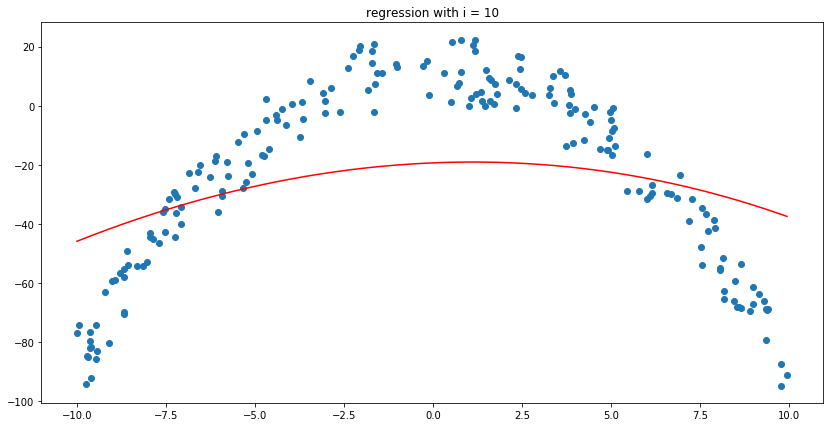
\includegraphics[width=\linewidth]{4b3.png}\\